\documentclass[10pt,a4paper]{article}
\usepackage[utf8]{inputenc}
\usepackage[english]{babel}
\usepackage[T1]{fontenc}
\usepackage{amsmath}
\usepackage{amsfonts}
\usepackage{amssymb}
\usepackage{makeidx}
\usepackage{graphicx}
\usepackage{fourier}
\usepackage{listings}
\usepackage{color}
\usepackage{hyperref}
\usepackage[left=2cm,right=2cm,top=2cm,bottom=2cm]{geometry}
\author{Johannes Scheller, Vincent Noculak, Lukas Powalla}
\title{Computational Physics - Project 3}
\begin{document}
\lstset{language=C++,
	keywordstyle=\bfseries\color{blue},
	commentstyle=\itshape\color{red},
	stringstyle=\color{green},
	identifierstyle=\bfseries,
	frame=single}
\maketitle
\newpage
\tableofcontents
\newpage
\section{Execution}

\subsection{Gaussian quadrature}
Our first task was to calculate the integral in Cartesian coordinates by Gaussian quadrature using only Legendre polynomials. With this method, it is only possible to integrate a function on some finite interval $[a,b]$. Therefore, we had to replace the original integration limits $-\inf$ and $\inf$ by some appropriate values $-a$ and $a$. As it can be seen in fig. \ref{oneparticle}, the one-dimensional wave function of only one particle gets more or less zero at $r=2$. Therefore, we decided to chose $[-2,2]$ as the interval for our first trials.
\begin{figure}[h]
	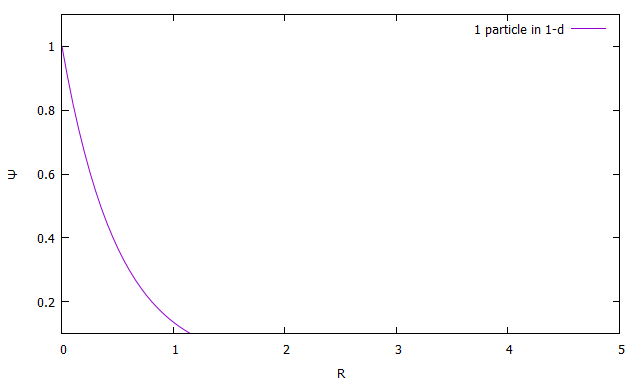
\includegraphics[width=\textwidth]{Psi.png}
	\caption{The one-dimensional wave function of one electron \label{oneparticle}}
\end{figure}

Our program reads in the desired number of grid points, $n$, and the desired integration limits $a$ and $b$. After that, it starts an algorithm to calculate the weights $w_i$ and zeros $x_i$ of a Legendre polynomial of the desired degree $n$ and to save them in arrays. This algorithm is taken from the source-code \glqq exampleprogram.cpp\grqq from the project folder for this course on Github. After calculating the weights and zeros, the algorithm performs a sextuple loop over the arrays and to sum up the weighted values of the function at those points and returns the result:
\begin{lstlisting}
double legendre(int n, double a, double b){
double * x = new double [n];
double * w = new double [n];
gauleg(a, b, x, w, n);
double integral = 0;
for (int i=0; i<n; i++){
for (int j=0; j< n; j++){
for (int k=0; k<n; k++){
for (int l=0; l<n; l++){
for (int y=0; y<n; y++){
for (int z=0; z<n; z++){
	integral += (w[i] * w[j] * w[k] * w[l] * w[y]* w[z]
				* function_cartesian(x[i], x[j], x[k], x[l], x[y], x[z]));
}}}}}}
return integral;
delete x;
delete w;
\end{lstlisting}
The function \emph{function\_cartesian} simply returns the function value at a given point.

In tab. \ref{results_leg}, you can see the results of this method for some different values of $n$ and some different intervals $[-a,a]$. It is very obvious that these results did not turn to be stable at all. Nevertheless, the computation time was already very high for $n=20$, as we had to perform roughly $n^6$ operations! Remember that the analytical value of the integral is $\frac{5\pi}{256}$.
\begin{table}[h]
	\caption{Results and computation time using Gauss-Legendre\label{results_leg}}
	\centering
\begin{tabular}{lcccr}
	$n$	&	$a=1$	&	$a=2$	&	$a=5$	&	time $t/\mathrm{s}$	\\\hline
	5	&	0.202983	&	0.354602	&	0.0423687	&	<0.1	\\
	10	&	0.151093	&	0.129834	&	0.0111647	&	0.235	\\
	20	&	0.16142	&	0.177065	&	0.0967888	&	15.896	\\
	25	&	0.163018	&	0.18911	&	0.240135	&	59.496	\\
	30	&	0.163214	&	0.185796	&	0.146371	&	182.404		
\end{tabular}
\end{table}

To improve the results, we tried calculating the integral with Gauss-Laguerre quadrature. The standard integration limits of Laguerre polynomials are $[0,\inf]$ and the polynomials are suited for functions of the form $x^\alpha\cdot \mathrm{e}^{-x}$. This fits perfectly to our case when we change to spherical coordinates:\\
The integral
\begin{equation}
\int_{-\infty}^{\infty} d\mathbf{r_1}d\mathbf{r_2}\mathrm{e}^{-4(r_1+r_2)}\frac{1}{|\mathbf{r_1}-\mathbf{r_2}}
\end{equation}
can now be written as
\begin{equation}
\int_{-\pi}^{\pi}\left(\int_{-\pi}^{\pi}\left(\int_{0}^{\pi}\left(\int_{0}^{\pi}\left(\int_{0}^{\infty}\left(\int_{0}^{\infty}\left(r_1^2r_2^2\sin(\theta_1)\sin(\theta_2)\mathrm{e}^{-4(r_1+r_2)}\frac{1}{|\mathbf{r_1}-\mathbf{r_2}}\right)dr_1\right)dr_2\right)d\theta_1\right)d\theta_2\right)d\phi_1\right)d\phi_2
\end{equation}
which perfectly fits to the form of Laguerre polynomials if we substitute $r_i'=4r_i$. Note that we have to change the Jacobian accordingly! Now we can solve the integral by applying Gauss-Laguerre quadrature for the two integrals over $r_i'$ and by using Gauss-Legendre for the integrals over the angles.

This program takes the same number of grid points as for Gauss-Legendre. Our algorithm again sets up the weights and zeros for both methods in arrays by using algorithms from the course folder on Github. Then it calculates the weighted function values in a sextuple for-loop, sums them up and returns the integral:
\begin{lstlisting}
double laguerre_legendre(int n){
double * xlag = new double[n+1];
double * wlag = new double[n+1];
double * xphi = new double[n];
double * wphi = new double[n];
double * xtheta = new double[n];
double * wtheta = new double[n];
double a, b;
a=0;
b=2*M_PI;
gauleg(a, b, xphi, wphi, n);
a=0;
b=M_PI;
gauleg(a, b, xtheta, wtheta, n);
//alpha=2 because of r^2 in Jacobian!
gauss_laguerre(xlag, wlag, n, 2.);
double integral=0;
for (int i=1; i<= n; i++){
for (int j=1; j<= n; j++){
for (int k=0; k<n; k++){
for (int l=0; l<n; l++){
for (int y=0; y<n; y++){
for (int z=0; z<n; z++){
	//integral+=(laguerre weights)*(legendre weights*function value)*(Jacobian)
	//NOTE: Substituted r_1 and r_2 by r_1'=4*r_1 and r_2'=4*r_2!
	//Same in "function_spherical"! Changes Jacobian!
	integral+=((wlag[i]*wlag[j])*(wphi[k]*wphi[l]*wtheta[y]*wtheta[z]
	*function_spherical(xlag[i], xlag[j], xphi[k], xphi[l], xtheta[y], xtheta[z]))
	*(sin(xtheta[y])*sin(xtheta[z])))/4096;
}}}}}}
delete wphi;
delete wtheta;
delete wlag;
delete xphi;
delete xtheta;
delete xlag;
return integral;
}
\end{lstlisting}
Note that in this case the function \emph{function\_spherical} only contains the parts of the function that are not absorbed in the Laguerre weights! Also look at the new Jacobian and the factors we had to add as we made the substitution $r_i'=4r_i$.

In table \ref{results_lag}, you can see the results of the Gauss-Laguerre quadrature. They converge much faster than the results we obtained with 'brute force' Gauss-Legendre and lead to a higher precision. Note that they still need a long computation time!

\begin{table}[h]
	\caption{Results and computation time using Gauss-Laguerre\label{results_lag}}
	\centering
	\begin{tabular}{lcr}
		$n$	&	Integral	&	time $t/\mathrm{s}$	\\\hline
		5	&	0.17345	&	0.017	\\
		10	&	0.186457	&	0.381	\\
		20	&	0.191082	&	26.538	\\
		25	&	0.191741	&	100.167	\\
		30	&	0.192114	&	298.406	
	\end{tabular}
\end{table}

\section{Comparison and discussion of the results}

\section{Source-code}
\end{document}